
\newcommand{\mycolor}{black}

\tikzsetnextfilename{adjacency1}

\centering
\resizebox{1\columnwidth}{!}{
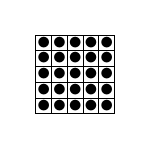
\begin{tikzpicture}[yscale=-1] 

\pgfmathsetmacro{\nn}{5} % time points


%% control labels
\foreach \i in {1,...,\nn}{
	\foreach \j in {1,...,\nn}{
		\pgfmathsetmacro{\x}{0.2*\i};
		\pgfmathsetmacro{\y}{0.2*\j};
		% \node () at (\x,\y) {$\bullet$};
        \ifthenelse{\i<\j}{ \node () at (\x,\y) {$\bullet$}; }{}
        \draw[\mycolor](\x-0.1,\y-0.1) -- (\x+0.2-0.1,\y-0.1) -- (\x+0.2-0.1,\y+0.2-0.1) -- (\x-0.1,\y+0.2-0.1) -- (\x-0.1,\y-0.1);
} }



\end{tikzpicture}
}



